\begin{enumerate}[label=\thesection.\arabic*.,ref=\thesection.\theenumi]

\item
 The open-loop transfer function of a plant in a unity feedback configuration is given as 
\begin{equation}
    G(s) = \dfrac{K(s+4)}{(s+8)(s^{2}-9)}
\end{equation}
 The value of the gain $K(>0)$ for which $-1 + j2$ lies on the root locus is
    
  

\solution
  The closed loop transfer function for a negative feed back system is:
  \begin{equation}
      F(s) = \dfrac{G(s)}{1+G(s)H(s)}
  \end{equation}
Since it is a unity feed back system, $H(s) = 1$, and now using the characteristic equation at $s_{1} = -1 + j2$
\begin{equation}
1 + G(s_{1})H(s_{1}) = 0
\end{equation}
\begin{equation}
 G(s_{1}) = -1
\end{equation}
\begin{equation}
 |G(s_{1})| = 1
\end{equation}


\begin{equation}
    G(s_{1}) = \dfrac{K(s_{1}+4)}{(s_{1}+8)(s_{1}^{2}-9)}
\end{equation}
\begin{equation}
    G(s_{1}) = \dfrac{K(s_{1}+4)}{(s_{1}+8)(s_{1}+3)(s_{1}-3)}
\end{equation}
\begin{equation}
    G(s_{1}) = \dfrac{K(3+j2)}{(7+j2)(2+j2)(-4+j2)}
\end{equation}
\begin{equation}
    |G(s_{1})| = \dfrac{K\sqrt{13}}{\sqrt{51}\sqrt{8}\sqrt{20}} = 1
\end{equation}
\begin{equation}
    K = 25.05
\end{equation}


\begin{equation}
    F(s) = \dfrac{25.05(s+4)}{s^{3}+8s^{2}+16.05s+28.2}
\end{equation}

    $Z_{1}=-4, P_{1}=-6.13, P_{2}=-0.93+j1.93, P_{3}=-0.93-j1.93$


\begin{figure}
\centering
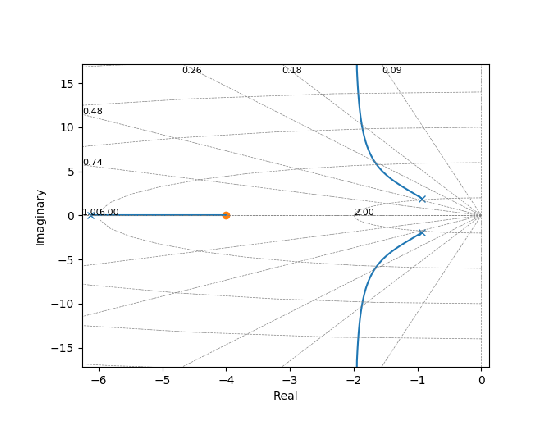
\includegraphics[width=\columnwidth]{figs/ee18btech11052.eps}
\caption{Root locus plot for verification}
\end{figure}


\begin{lstlisting}
codes/ee18btech11052.py
\end{lstlisting}
    
\end{enumerate}

